\documentclass[11pt]{article}

\usepackage{graphicx}
\usepackage{geometry}
\usepackage{tikz-cd}
\usepackage{amsmath}
\usepackage{amssymb}
\usepackage{authblk}
% \usepackage{subfigure}
\usepackage{graphicx}
\usepackage{caption}

\usepackage{listings}
\usepackage{xcolor}

\definecolor{codegreen}{rgb}{0,0.6,0}
\definecolor{codegray}{rgb}{0.5,0.5,0.5}
\definecolor{codepurple}{rgb}{0.58,0,0.82}
\definecolor{backcolour}{rgb}{0.95,0.95,0.92}

\lstdefinestyle{mystyle}{
    backgroundcolor=\color{backcolour},   
    commentstyle=\color{codegreen},
    keywordstyle=\color{magenta},
    numberstyle=\tiny\color{codegray},
    stringstyle=\color{codepurple},
    basicstyle=\ttfamily\footnotesize,
    breakatwhitespace=false,         
    breaklines=true,                 
    captionpos=b,                    
    keepspaces=true,                 
    numbers=left,                    
    numbersep=5pt,                  
    showspaces=false,                
    showstringspaces=false,
    showtabs=false,                  
    tabsize=2
}

\lstset{style=mystyle}



\geometry{a4paper,scale=0.8}
\title{Lab 3: DASH Based on Deep Q-Learning}
\author{Zhipeng Ye}
\affil{Department of Electrical and Electronic Engineering \\Xi’an Jiaotong-Liverpool University}
\begin{document}

\maketitle

\section{Introduction}
Video streaming has become the most popular source for broadcasting information on the internet. Dynamic Adaptive Streaming over HTTP(DASH) has become the dominant standard for video transmission since it was proposed.
DASH is a industrial approach for video streaming.

\begin{figure}[htbp]
    \centering
        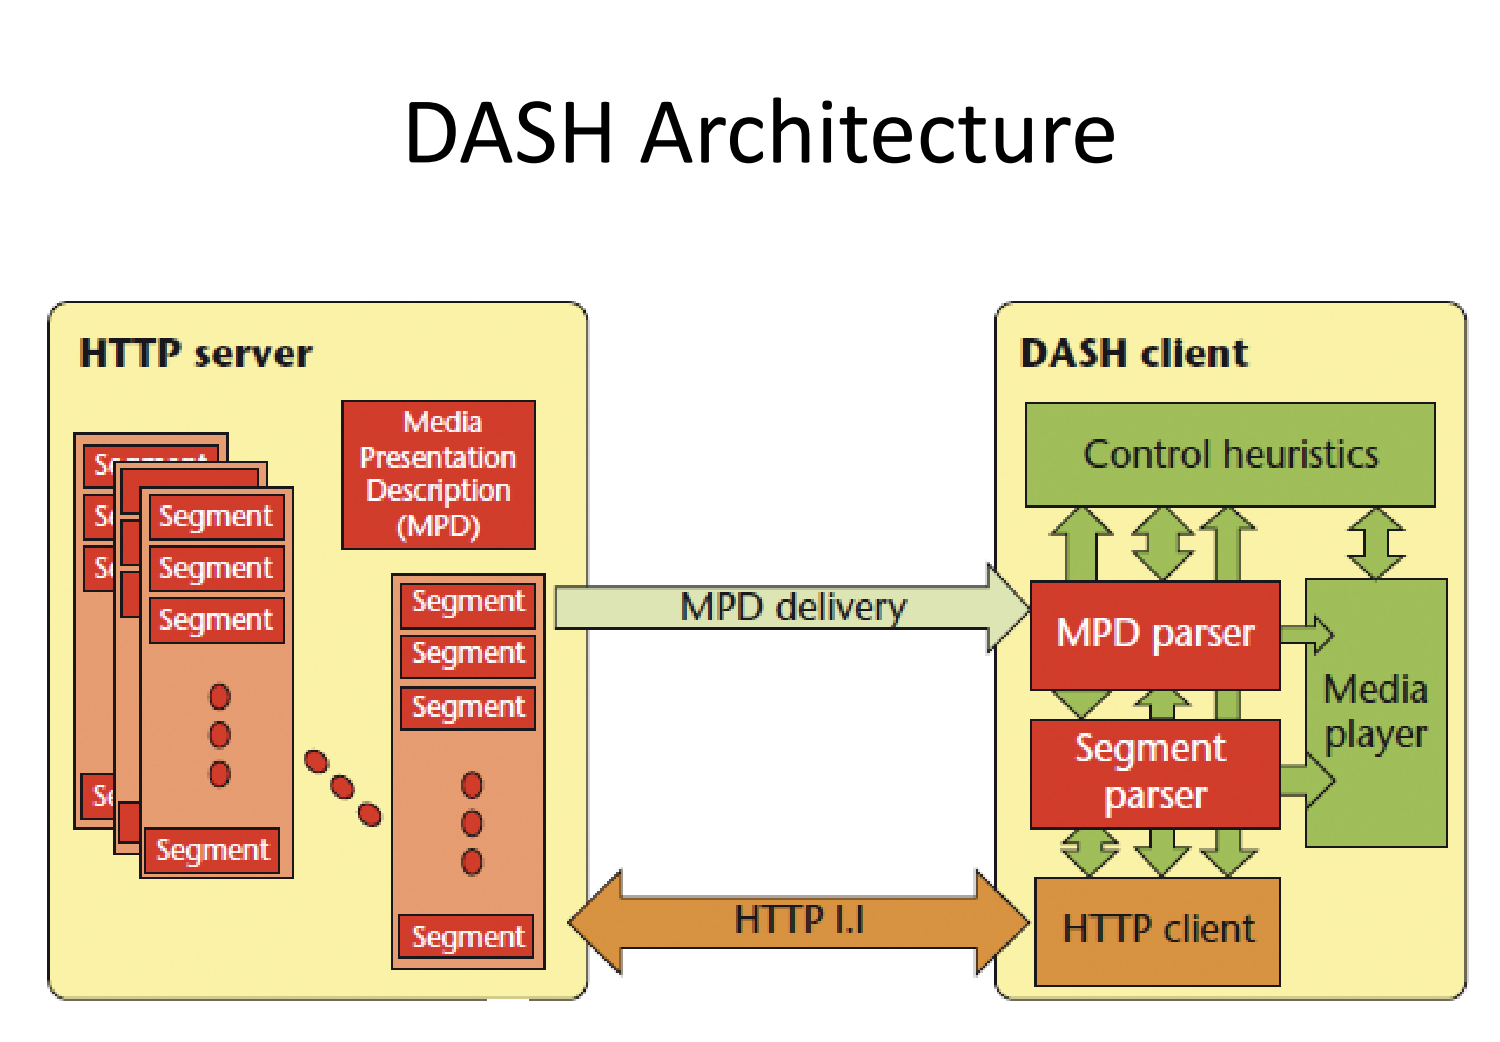
\includegraphics[width= 0.8\textwidth]{DASH.png}
    \caption{DASH Architecture}
    \label{DASH Architecture}
\end{figure}

As shown in Figure \ref{DASH  Architecture}, server divide the video content into segments, each segment can exist in different encoding forms.
Client can freely choose the media segments to be played and implement adaptive bitrate streaming technology. The seamless switching of different picture quality content provides a better playback experience.
\subsection{D-DASH}
All methods is proposed to optimize the Quality of Experience(QoE) for the current video and network conditions. Recently, some researchers commit themself on DASH adaption algorithm because of huge prospect of this domain.
D-DASH is a state of the art for dynamic adaption algorithm of DASH which combines Deep Learning and Reinforcement Learning. 
As we can see from Figure \ref{D-DASH},
This algorithm will give the appropriate suggestion quality of video based on the current state (previous suggestion quality level of video, previous suggestion quality size of video, buffer time, current bandwidth size). 
\begin{figure}[htbp]
    \centering
        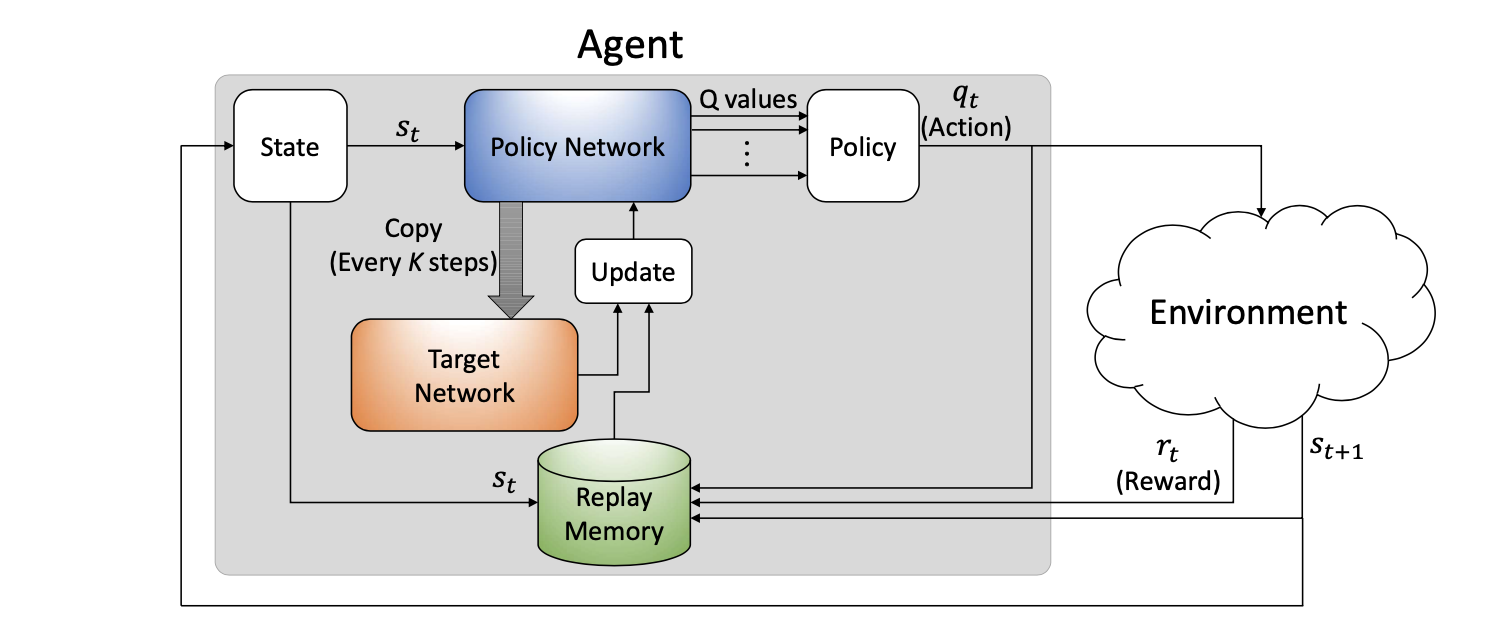
\includegraphics[width=0.9\textwidth]{d-dash.png}
    \caption{D-DASH Architecture}
    \label{D-DASH}
\end{figure}

D-DASH use advanced D-Q-Network technology of Reinforcement Learning, which combine Q-Learning and Deep Leaning network. 

Futhermore, It's necessary to figure out the difference between reinforcement learning and Deep Learning. 
Reinforcement learning is a algorithm to make decesion which maximize cumulative rewards and punishments.
Deep learning is a technology to classify or predict data based on previous data. D-Q-Network combine them and take advantages of their features due to the drawback of Q-learning.
Next, we will have detailed disscussion about the reinforce learning and Q-learning. 

\subsection{Reinforcement Learning and Q-learning}
Reinforcement learning is a bunch of algorithm to make machine learn how to make decision based on environment. Machine will take the action randomly, the algorithm will give the reward or punishments for each action. Machine will learn how to make decision to maximize the reward and minimize the punishments.
Q-learning is classical algorithm of Reinforcement Learning.
Q-learning use a table to store the all state and reward.

\section{Experiment}

\section{Conclusion}

\end{document}
